\chapter{vim语法总结}

需要使用setup_vim.sh来安装vim插件及配置,其有更强的IDLE功能,方便编辑。

\section{vim基础用法}
下面是基础运法,英文,懒得翻译,就这样看吧。

General 

Nearly all commands can be preceded by a number for a repeat count. eg. 5dd delete 5 lines 

Commands preceded by : are executed on the command line at the bottom of the screen 

:help help with any command 

By marker:  mx set mark x; 'x go to mark x ; '. go to position of last edit ;  ' ' go back to last point before jump 

Scrolling: 

ctrl-f forward full screen; ctrl-b backward full screen 

ctrl-d down half screen; ctrl-u up half screen 

ctrl-e scroll one line up; ctrl-y scroll one line down 

zz centre cursor line 


Changing 

c<motion> changes text in the direction of the motion: ci( change inside parentheses) cw change word; C change to end of line; cc change whole line 

d<motion> deletes in the direction of the motion: dw delete word; D delete to end of line; dd delete whole line 

Blocks 

v visual block stream; V visual block line; ctrl-V visual block column 

most motion commands extend the block to the new cursor position; o moves the cursor to the other end of the block; d or x cut block into paste buffer; y copy block into paste buffer; > indent block; < unindent block; gv reselect last visual block 

Global 

:\%s/foo/bar/g substitute all occurrences of "foo" to "bar" 

\% is a range that indicates every line in the file, /g is a flag that changes all occurrences on a line instead of just the first one 

Searching 

/ search forward; ? search backward 

* search forward for word under cursor; \# search backward for word under cursor 

n next match in same direction; N next match in opposite direction 

fx forward to next character x; Fx backward to previous character x 

; move again to same character in same direction; , move again to same character in opposite direction 

Files 

:w write file to disk; \textit{:w name} write file to disk as name 

ZZ write file to disk and quit 

:n edit a new file; :n! edit a new file without saving current changes 

:q quit editing a file; :q! quit editing without saving changes 

:e edit same file again (if changed outside vim) 

:e . directory explorer 

Windows 
ctrl-w+n new window, ctrl-w+j down to next window; ctrl-w+k up to previous window 

ctrl-w+ _  maximize current window; ctrl-w+= make all windows equal size 

ctrl-w++ increase window size; ctrl-w+- decrease window size 

Source Navigation 

\% jump to matching parenthesis/bracket/brace, or language block if language module loaded 

gd go to definition of local symbol under cursor; ctrl-o return to previous position 

ctrl-t return to previous position (arbitrary stack of positions maintained) 

ctrl-n (in insert mode) automatic word completion 

Show local changes 

Vim has some features that make it easy to highlight lines that have been changed from a base version in source control. I have created a small vim script that makes this

\begin{figure}[!ht]
    \centering
    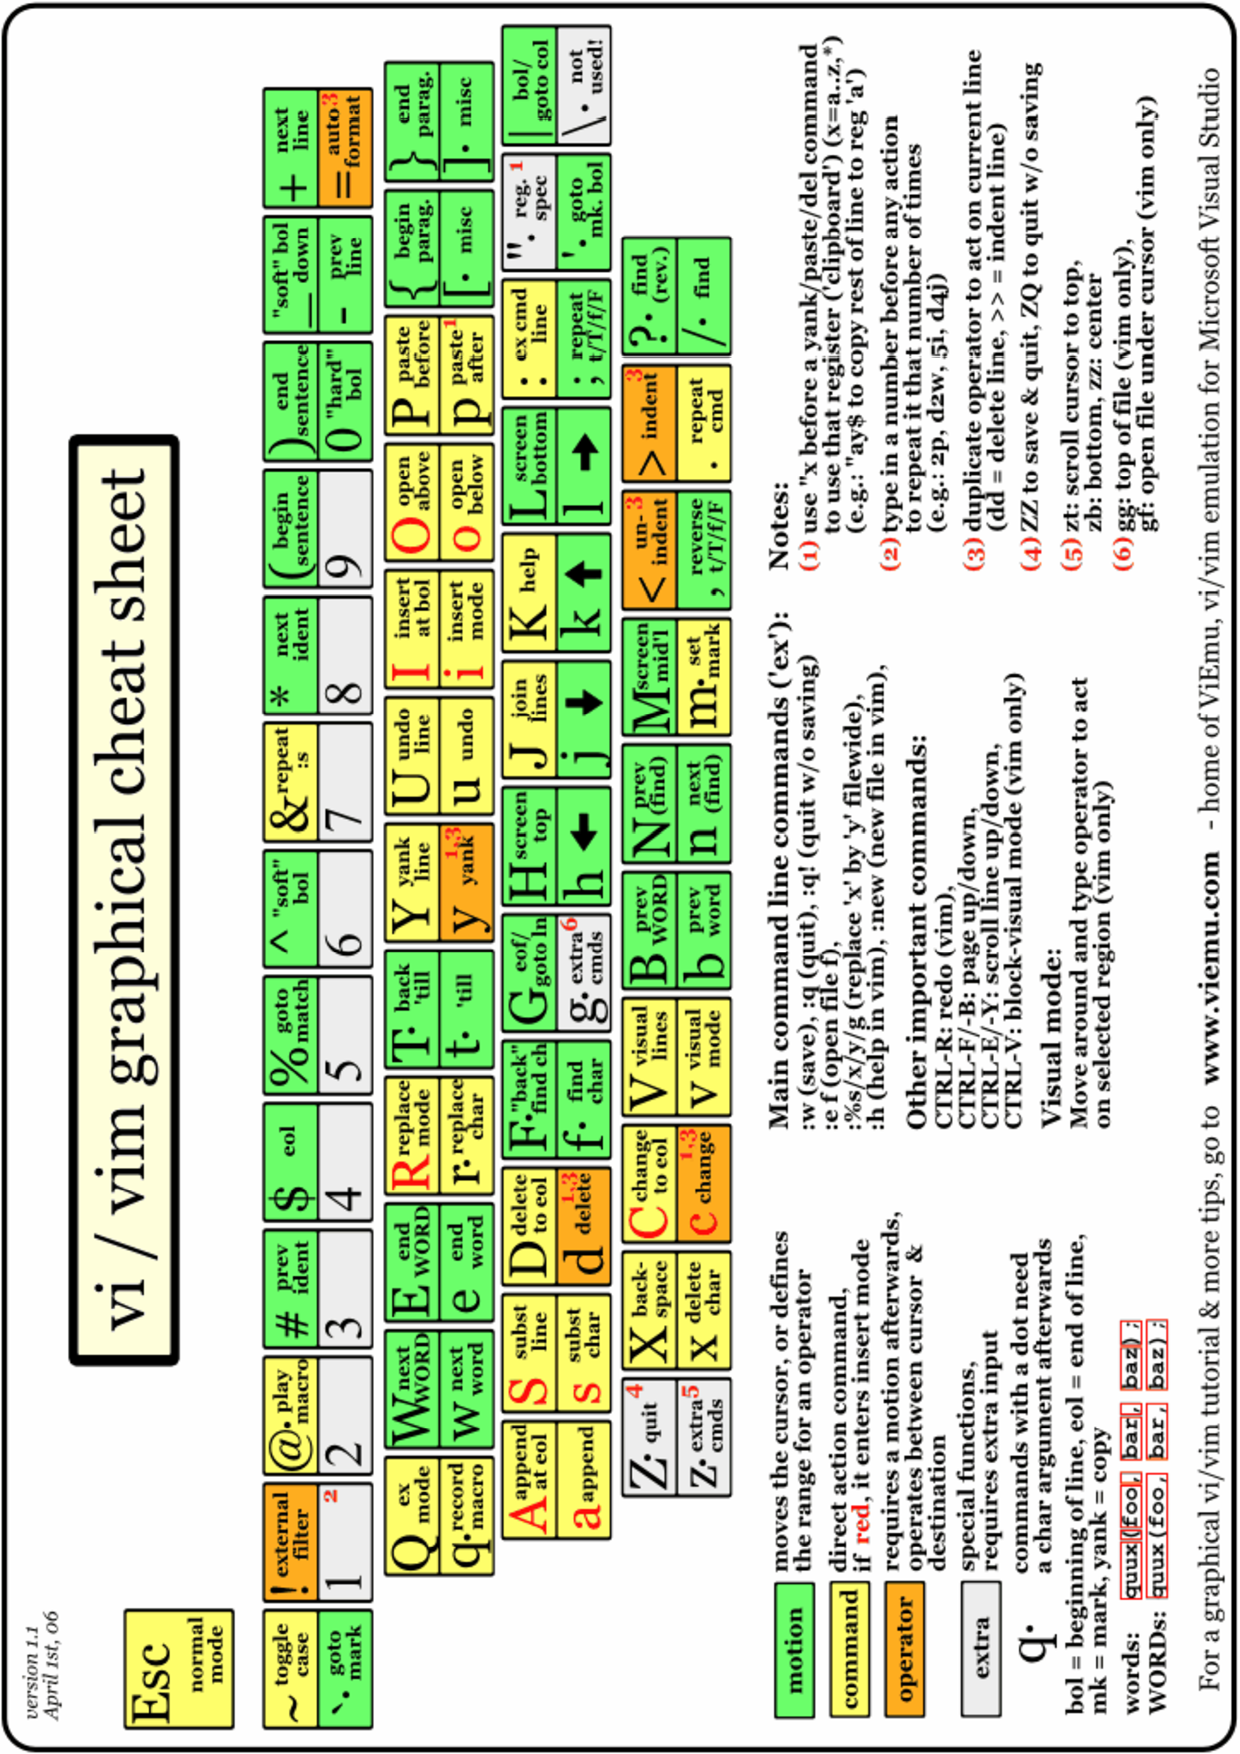
\includegraphics[width=0.8\textwidth]{vim/i3iyY.pdf}
    \caption{\label{Fig:vim-graphical sheet} vim-graphical sheet}
\end{figure}

\begin{lstlisting}
:sort  对文本排序 
:!g/^faile\$/d   搜索匹配行并删除
:\% g/^#/d       删除含有“#”开头的行 
:\% g/^\$/d      删除空行 
:\% v/pattern/d    删除不含该字符串的行 
:\% g!/pattern/d   删除不含该字符串的行 
:\%s/^.*\(pattern\).*\$/\1/g    对每行只保留匹配内容而删除这一行中的其它内容,
:g/pattern/d 删除包含特定字符串的行,
:\%s/^.*pattern.*\n//c     删除包含特定字符串的行,每次删除前都提示 
:s/vivian/sky/ 替换当前行第一个 vivian 为 sky 
:s/vivian/sky/g 替换当前行所有 vivian 为 sky 
:n,\$s/vivian/sky/ 替换第 n 行开始到最后一行中每一行的第一个 vivian 为 sky 
:n,\$s/vivian/sky/g 替换第 n 行开始到最后一行中每一行所有 vivian 为 sky ; n 为数字,若 n 为 .,表示从当前行开始到最后一行 
:\%s/vivian/sky/  (等同于 :g/vivian/s//sky/) 替换每一行的第一个 vivian 为 sky 
:\%s/vivian/sky/g (等同于 :g/vivian/s//sky/g) 替换每一行中所有 vivian 为 sky 
\end{lstlisting}

处理字符串: /123/456/789/109/example.txt, 怎么删除到最后一个/,然后得到example.txt ? 答案是 \textit{0dte}, 说明:0到行首, dte   删到第一个e 

处理字符串: /123/456/789/ef/109/example.txt, 怎么删除到最后一个/,然后得到example.txt ?  答案是 \textit{\$T/d0  } 说明:\$ 到行尾, T/从后往前搜到第一个/ 
,  d0删到行首. 或者 \textit{d/ex}然后回车 , 说明:d删除;  /ex搜到第一个ex 
 
上面所有例子都是以/为分隔符,事实上分隔符是任意的,可以使用任何符号,比如有人喜欢使用\#号,也有人喜欢使用+号 



显示重复行
\begin{lstlisting}
syn clear Repeat | g/^\(.*\)\n\ze\%(.*\n\)*\1$/exe 'syn match Repeat "^' . escape(getline('.'), '".\^$*[]') . '$"' | nohlsearch  
 \end{lstlisting}
sort by column  
\begin{lstlisting}
:%!sort -k2nr
\end{lstlisting}

\section{切分窗口}
横向切割 \textit{:new FILENAME } or \textit{:split FILENAME }

纵向切割  \textit{:vsplit FILENAME}

窗口之间切换 原始情况下使用Ctrl + w + (h/j/k/l)来上下左右切换   

使用本目录下的配置后可以使用 Ctrl + (hjkl)上下左右切换窗口 

Ctrl + n 打开目录窗口


批量删除,以批量注释
命令模式下按 ctrl + v  移动光标选中需要修改的行,然后按x 或者 d 删除该内容或者按 I 或 A 进入编辑模式然后增加内容然后按esc退出后便可以看到所选区域都有显示

vim 下在编辑模式下也有自动补全功能便不是tab键,而是 ctrl + n,
ctrl + o 跳到上一次修改的地方

\section{vim高级用法}

区域选择 

其格式为 <action>a<object> 和 <action>i<object> 
action可以是任何的命令,如 d (删除), y (拷贝), v (可以视模式选择)。 
object 可能是: w 一个单词, W 一个以空格为分隔的单词, s 一个句字, p 一个段落。也可以是一个特别的字符:单引号,双引号,小括号,中括号,大括号。 
举例: daw 删除一个单词

块操作 

命令模式下按 ctrl + v 移动光标选中需要修改的行(区域), 
然后按x 或者 d 删除该内容
批量在行首增加内容: 
ctrl + v >> 0 >> I >> 写下想增加的内容 >>Esc 


宏录制 
qa 开始录制宏,并把宏的名字取名为a 
q 停止录制宏 
@a 用@来调用宏并执行 
@@ 快捷的执行最新操作的宏 

\section{vim插件使用}

执行setup_vim.sh,便会安装好现有插件,这仅限自己使用。

